\subsubsection{Generalidades}

Os itens listados nesta seção referem-se a todos os itens subsequentes de quadros apresentados a seguir.

\begin{enumerate}
	\item Ser instalado em local de fácil acesso e manutenção
	\item Preferencialmente e sempre que possível instalados nos pavimentos técnicos
	\item Os quadro elétricos devem ser identificados através de uma plaqueta impressa em adesivo de PVC colada no objeto a ser identificado ou impressa em adesivo de PVC colado em chapa de PVC de 2mm a ser fixado no objeto a ser identificado. As dimensões devem seguir as especificações abaixo(cotas em mm):
	\begin{figure}[H]
		\centering
	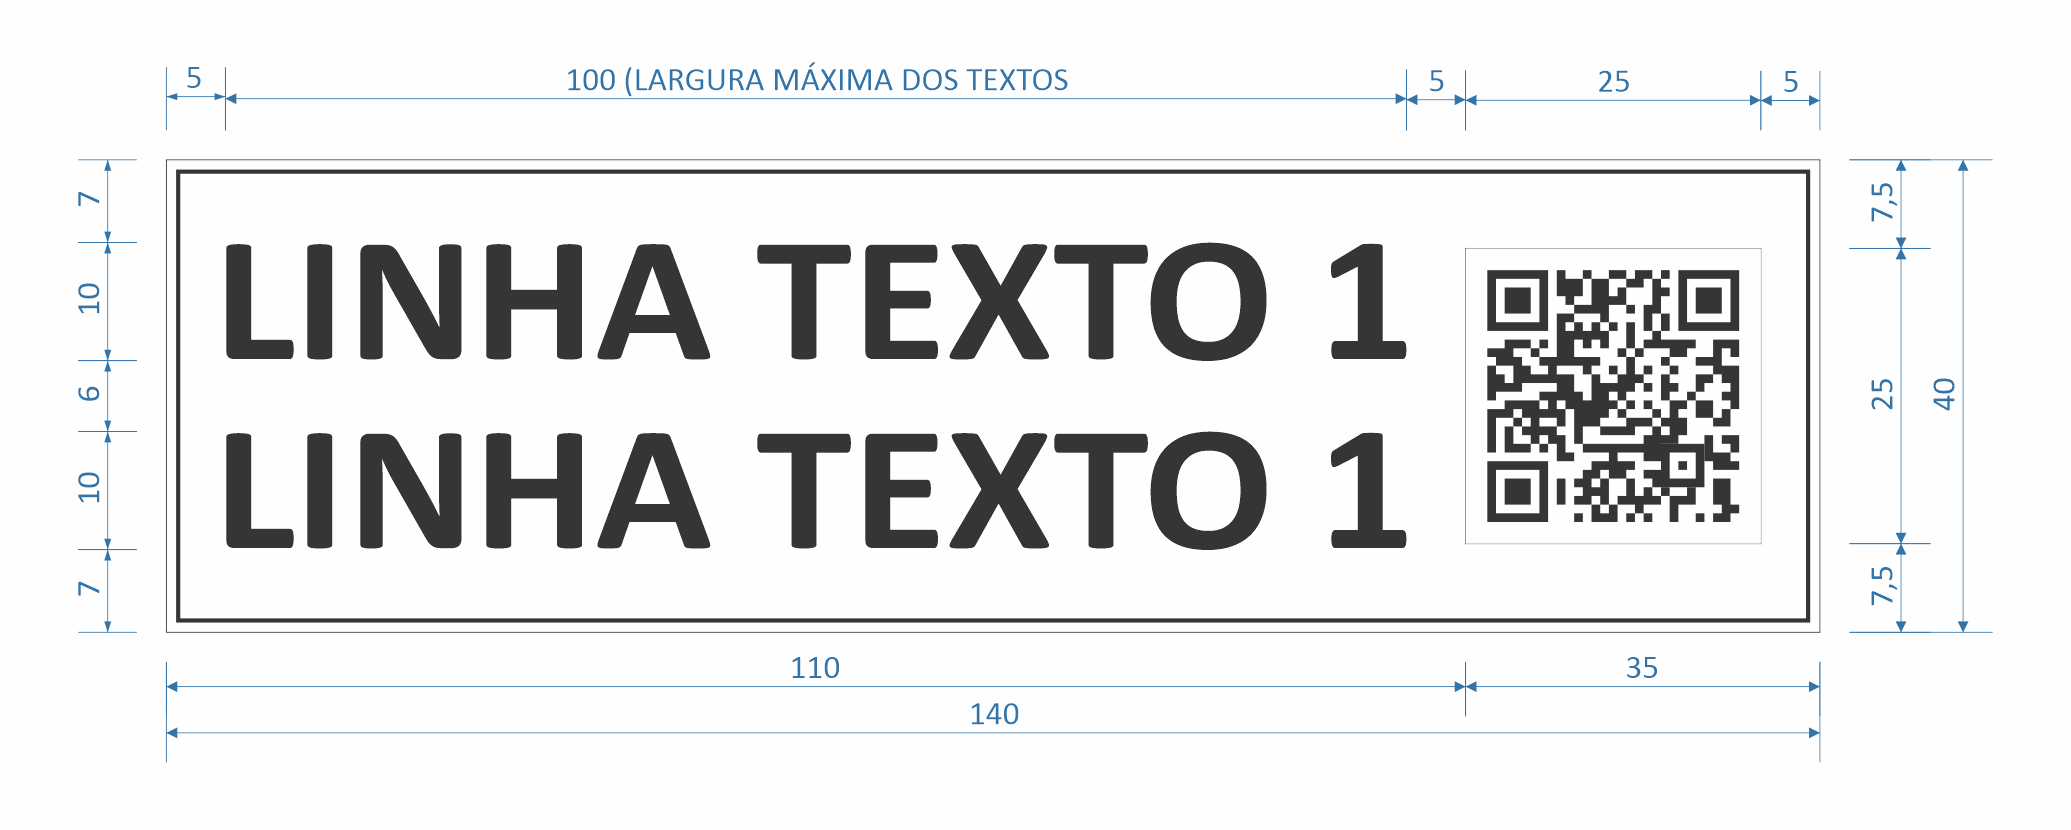
\includegraphics[scale=.85]{Figures/6. Distribution/PLACAS_QUADROS_ELETRICA-01.png}
	\caption{Plaqueta de identificação de quadros elétricos}
	\label{fig:plaqueta01}
	\end{figure}
\end{enumerate}